\subsection{BraggNN}\label{subsec:braggnn}

TODO: stuff about BraggNN

\subsection{Translating DNNs}\label{subsec:translatingdnns}
Our design methodology for BraggNN winds its way through several levels of abstraction and tooling:

\begin{enumerate}
	\item A conventional PyTorch representation;
	\item A JIT traced representation called TorchScript;
	\item Several, successively lower-level, MLIR representations;
	\item A LLVM IR representation;
	\item A RTL representation.
\end{enumerate}

We quickly review the relevant concepts of each level of abstraction.

\subsubsection{PyTorch/TorchScript}\label{subsec:pytorch}

Typically DNN models are represented in terms of high-level frameworks implemented within general purpose programming languages.
Such frameworks are widely used because of their ease of use and large library of example implementations of various DNN model architectures.
Two such frameworks are TensorFlow and PyTorch.
BraggNN is implemented within PyTorch.
DNNs are developed within PyTorch using the \emph{define-by-run} methodology (also known as \emph{eager mode}).
Using this methodology, the developer writes conventional Python code that describes the sequential execution of the high-level operations comprising the model, and the dataflow graph (for purposes of backprop/autodiff) is simultaneously defined and constructed at runtime.
With respect to the developer, define-by-run, which is not unique to PyTorch, enables fast iteration at development time, at the cost of some runtime performance (when compared with frameworks that require statically specifying the model).

With respect to the kind of program analysis necessitated by our translation of BraggNN, there is another cost to define-by-run DNN specification: the dataflow graph (DFG) is never fully materialized\footnote{``...instead, every intermediate result records only the subset of the computation graph that was relevant to their computation.''~\cite{paszke2017automatic}} and the control flow graph (CFG) is difficult to extract from the semantics of the general purpose language (Python in the case of PyTorch).
The PyTorch organization, having recognized these issues (in the course and context of their own deployment projects), in recent years has implemented a Single Static Assignment (SSA) intermediate representation (IR), called TorchScript (TS) and concomitant tracing mechanism (colloquially referred to as the TS JIT compiler) to produce TS from conventionally defined PyTorch models.
The exact operation of this tracing mechanism is beyond the scope of our work\footnote{\url{https://github.com/pytorch/pytorch/wiki/PyTorch-dispatcher-walkthrough}}, but two of its limitations, as they pertain to our work, merit discussion.
Firstly, much like other JIT compilers, the TS JIT does not easily support control flow \footnote{(\inlinemlir{prim::If}, \inlinemlir{prim::While}) primitives are part of the TS IR specification but they are not captured by tracing (though they are captured by \inlinepython{torch.jit.script}).} in the DNN model specification.
In reality, even if control flow were supported, we would still be unable to effectively support such dynamism since FPGAs do not (currently) support runtime reconfiguration~\cite{reconfigfpga}.
Secondly, TS IR does not always produce fully refined tensor types.
That is to say, tensor shapes, as they appear in the TS IR, are either absent or specified with symbolic dimensions~\cite{10.1145/3211346.3211348}; for much the same reason as in the case of control flow, our approach necessitates fully known tensor shapes, and for this we rely on explicit annotation.

In practice neither of these limitations is a serious impediment to deployment; \commnt{run the test}{only x/y models in the standard benchmark torchbench} exhibit either or both types of dynamism, and our target model, BraggNN, exhibits neither form of dynamism.
\begin{figure*}
  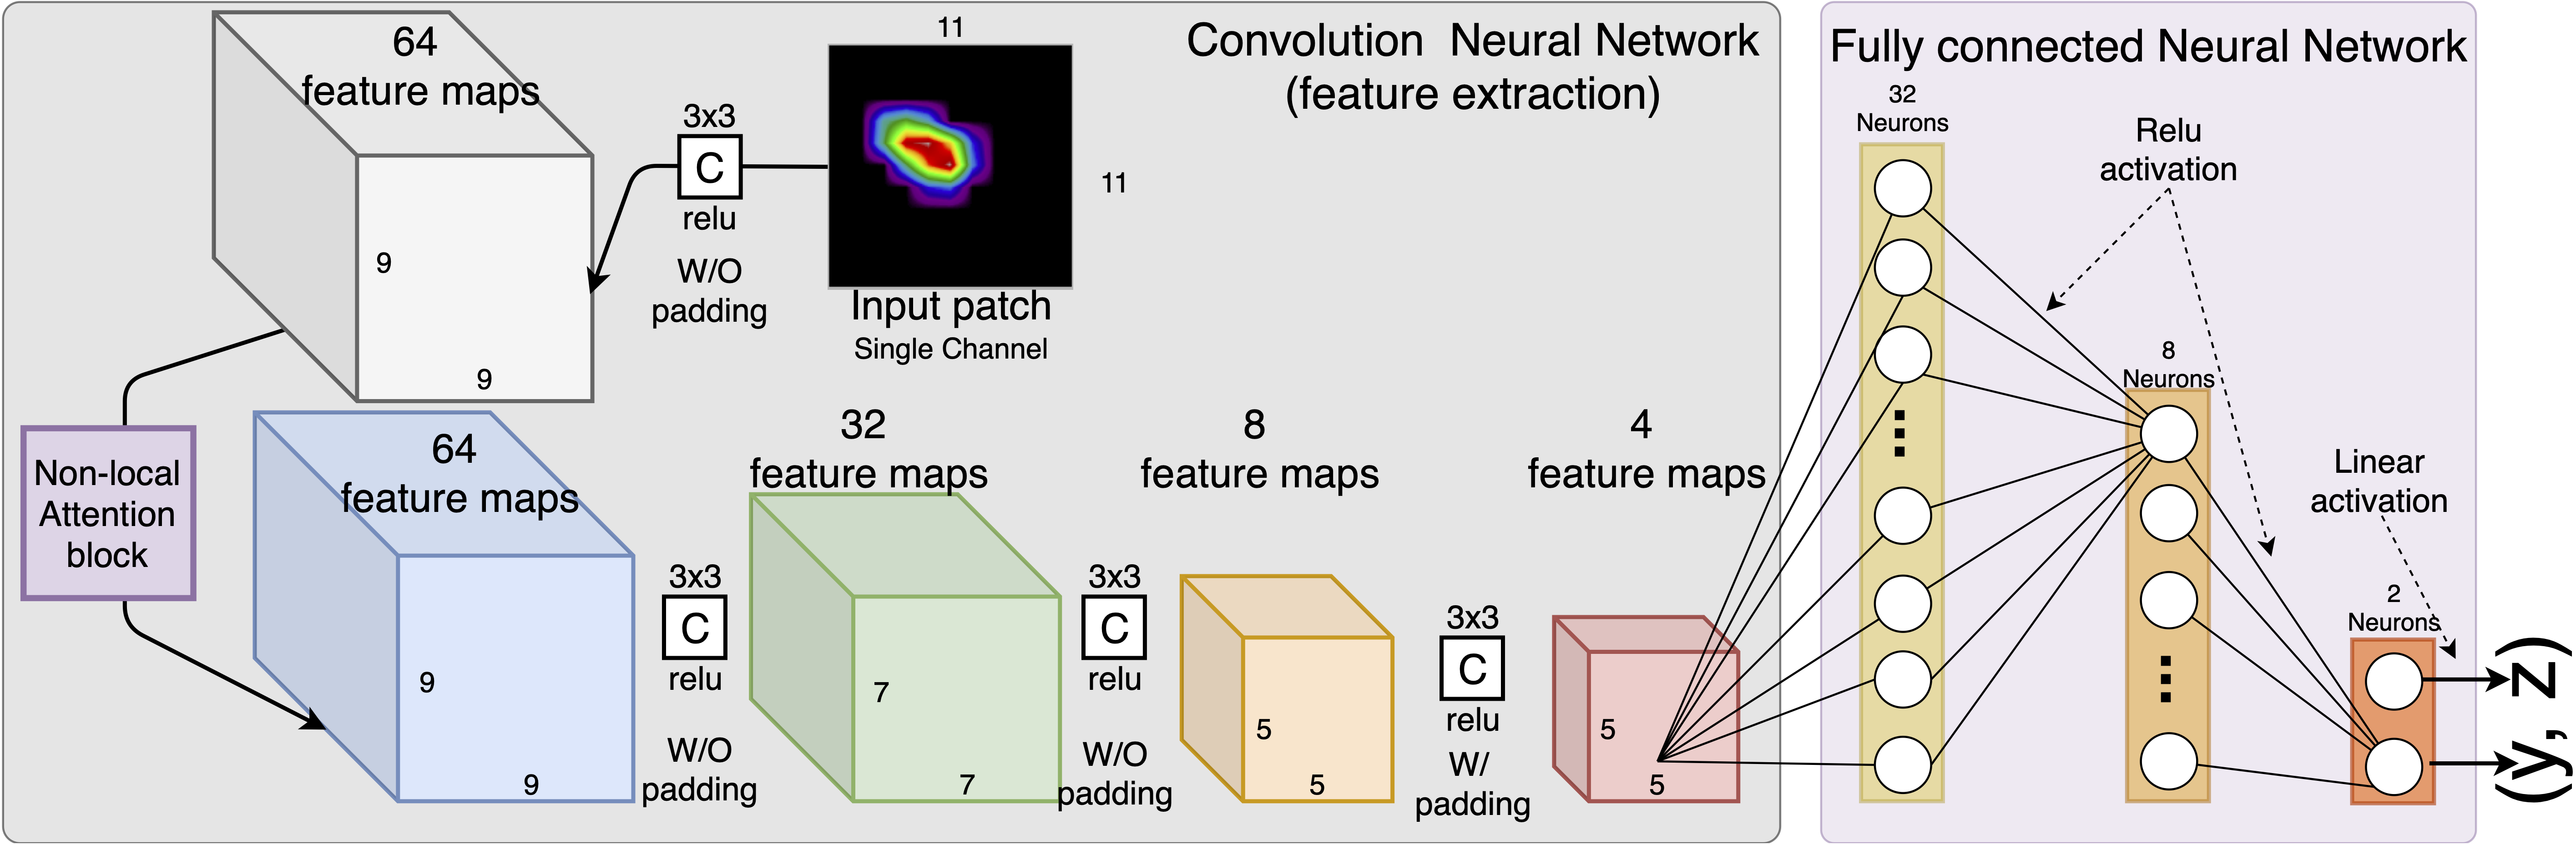
\includegraphics[width=\textwidth]{figures/BraggNN}
  \caption{This is a placeholder.}
\end{figure*}
Lowering from PyTorch to TS IR allows us to perform many useful analyses and transformations on BraggNN that would be extremely difficult (or impossible) on the original representation;
basic optimizations like dead code elimination and constant propagation are supported by TS's graph rewriting functions.
In addition, PyTorch also supports at least two kernel fusion~\cite{10.1145/2688500.2688521} tools (NNC fuser and nvfuser).
Such transformations are critical for achieving peak performance on CPUs and hardware accelerators alike but for our purposes, deployment to application specific hardware, we require a broader collection of transformations.
To this end, we turn to a recent addition to the compiler ecosystem.

\subsubsection{MLIR}\label{subsec:mlir}

Multi-level Intermediate Representation (MLIR)~\cite{https://doi.org/10.48550/arxiv.2002.11054} is a new approach to building reusable and extensible compiler infrastructure.
MLIR is composed of a set of \emph{dialect} IRs, subsets of which are mutually compatible, either outright or by way of translation/legalization.
The various dialects aim to capture and formalize the semantics of compute intensive programs at varying levels of abstraction, as well as namespace related sets of IR transformations/optimizations (called \emph{passes}).
Our entrypoint into this compiler framework is the Torch dialect~\cite{torch-mlir}, a high-fidelity mapping from TS IR to MLIR native IR, which, in addition to performing the translation to MLIR, provides for us the necessary shape refinement mentioned above.

While Torch dialect acts as a thin shim around TS IR and does little "heavy lifting", the same cannot be said for other dialects in MLIR.
For example, the linalg dialect is designed to address the hierarchical optimization problem, wherein the goal is to enable code generation of efficient code or dispatch to existing, previously optimized, kernel code, without sacrificing ease of use and performance for either path.
Practically speaking, this entails representations of common mathematical operations, such as \inlinepython{matmul}, \inlinepython{conv}, and \inlinepython{batchnorm}, explicitly declaring semantics that are traditionally obtained only through compiler analysis (such as memory dependency) and transformations on such operations completely preserving such semantics.

We make extensive use of the linalg dialect as an intermediary between lower-level dialects, such as the affine and structured control flow dialects, and Torch dialect.
The structured control flow dialect is a straightforward formalization of control flow primitives, such as conditionals and loops, so we do not discuss it in great detail.
The affine dialect, on the other hand, provides a formalization of semantics that lend themselves to polyhedral compilation techniques~\cite{polyhedral-mlir}, i.e., techniques that make dependence analysis and loop transformations efficient and reliable.

The next step in the lowering is LLVM IR, an IR that is, technically speaking, not an MLIR dialect; the purpose of further lowering to LLVM IR is to produce a representation of BraggNN that high-level synthesis tools can consume.
We Briefly discuss the role of HLS in the translation process.

\subsubsection{High-Level Synthesis and Down}\label{subsec:hlsdown}

High-level synthesis tools produce RTL descriptions of digital designs from high-level representations, such as C or C++~\cite{10.1145/2514740, ferrandi2021bambu} or LLVM IR.
In particular, Xilinx's Vitis HLS, based on the Autopilot project~\cite{Zhang2008}, recently enabled passing LLVM IR to the tool, rather than C/C++.
Given a high-level, procedural, representation, HLS performs performs three functions, in order to produce a corresponding RTL design:
\begin{enumerate}
	\item HLS schedules operations (such as \mintinline{mlir}{fmult}, \mintinline{mlir}{fadd}, \mintinline{mlir}{load}, \mintinline{mlir}{store}) in order to determine which such operations should occur during each clock-cycle. A schedule depends on three parameters:
	      \begin{itemize}
		      \item The topological ordering of the DFG/CFG of the procedural representation (i.e., the dependencies of operations on results of other operations and resources);
		      \item The completion time for each operation;
		      \item The user's desired clock rate/frequency;
	      \end{itemize}
	\item HLS associates high-level operations to particular RTL instantiations (called \emph{binding}) for those operations; for example whether to associate an add operation followed by a multiply operation to two separate digial signal processors (DSP) instances, or whether to associate them both with a single DSP instance (configured to perform fused-multiply-add);
	\item HLS builds an FSM that cycles (transitions from state to state) through the sequence of operations in the schedule.
\end{enumerate}

In addition to fulfilling these three fundamental tasks, high-level synthesis tools such as Vitis, Bambu~\cite{ferrandi2021bambu}, LegUp~\cite{10.1145/2514740} perform standard compiler optimization passes on the IR (that they either receive or produce internally).
Optimization passes such as store-load forwarding, common subexpression elimination, and constant propagation.
Loop-unrolling and tiling are also performed at the behest of the user.
Note that the scheduling problem solved by HLS is reducible an integer programming problem~\cite{tuprints9272}, instance of which are generally NP-hard.
For certain instances, the scheduling problem can be reformulated as a system of difference constraints.
Such a formulation induces a unimodular matrix representation of the constraint system which is amenable to Bellman-Ford $O(n^2 + mn)$\commnt{this is phrased poorly - unimodular guarantees you integral solutions to the LP but also gives you the shortest path analogy property}{ for checking consistency of a solution (essentially the shortest path problem) }and an LP approach for optimizing the critical path~\cite{1688836}.
Thus, ostensibly, HLS tools solve computationally intensive problems in order to produce a RTL description of a high-level representation of a DNN.
At the RTL level of abstraction, there remain two more steps prior to being able to actually deploy to an FPGA; one of them being a final lowering, so called logic synthesis, and the other being Place and Route (PnR).

Logic synthesis is the process of mapping RTL to actual hardware primitives on the FPGA (so called \emph{technology mapping}), such as lookup tables (LUTs), registers, and DSPs (in cases where they haven't been explicitly instantiated).
Logic synthesis produces a network list (netlist) describing the logical connectivity of various parts of the design.
For example,
\begin{longlisting}
	\inputminted{verilog}{sources/always.v}
	\caption[Long Code Example]{A long code example which will break across pages.}
	\label{lst:long}
\end{longlisting}
\noindent corresponds to a state of an FSM during which the registers \inlinev{reg_1608}, \inlinev{reg_1613}, \inlinev{reg_1618} are updated with new values from wires (\inlinev{fu_1076_p2}, \inlinev{notrhs18_fu_1082_p2}, \inlinev{fu_646_p2}).
Assuming these registers are updated in other FSM states (from differing wires), this logic will synthesize to multiplexers (or possibly multiplexer trees, depending on how many different input wires feed these same registers).
Such multiplexers are actually implemented using Lookup Tables (LUTs) of varying sizes and multiplcities.
Another relevant concern is the implementation of floating point operations in terms of DSPs; depending on user parameters and other design features, DSP resource consumption for floating point multiplication and addition can differ greatly.
The number of LUTs and DSPs that a high-level representation of a DNN corresponds to is relevant to both the performance and feasibility of that DNN when deployed to FPGA (more on this in Section~\ref{subsec:parallel-toposort-scheduling}).

Finally, after the netlist has been produced, the entire design undergoes PnR.
The goal of PnR is to determine which configurable logic block within an FPGA should implement each of the units of logic required by the digital design.
PnR algorithms need to minimize distances between related units of functionality (in order to minimize wire delay), balance wire density across the entire fabric of the FPGA (in order to reduce route congestion), and maximize the clock speed of the design (a function of both wire delay, logic complexity, and route congestion).
The final, routed design, can then be deployed to the FPGA by producing a proprietary \emph{bitstream}, which is written to the FPGA.

In general, both of these final steps (logic synthesis and PnR) can only be performed by the proprietary tools of the hardware manufacturers (e.g., Vivado by Xilinx) and thus, from our perspective their inner workings are completely unknown.
Recently, open source alternatives for certain FPGAs have become available, thanks to herculean efforts made to reverse engineer the various bitstream formats of, for example, some of Xilinx's architectures~\cite{6546003}, and reimplement logic synthesis and PnR in open source.
Namely, ~\cite{wolf2013yosys} is a framework for Verilog RTL synthesis and Verilog to Routing~\cite{vtr} is a framework for place and route.
% It provides a basic set of synthesis algorithms for mapping to Xilinx and Lattice FPGA (as well as ASIC standard cells).
% We use Yosys as a basis of comparison for commercial tools and as a way to investigate the limitations of those tools (i.e., when Vivado fails, we can reason by analogy with Yosys, why it might've failed).